\chapter{Hello World}
\subsection{Anleitung}
\begin{table}[H]
\begin{tabular}{| p{5cm} | p{11cm} |}
\hline
Lorem ipsum dolor sit amet, consetetur sadipscing elitr, sed diam nonumy eirmod tempor invidunt ut labore et dolore magna 
&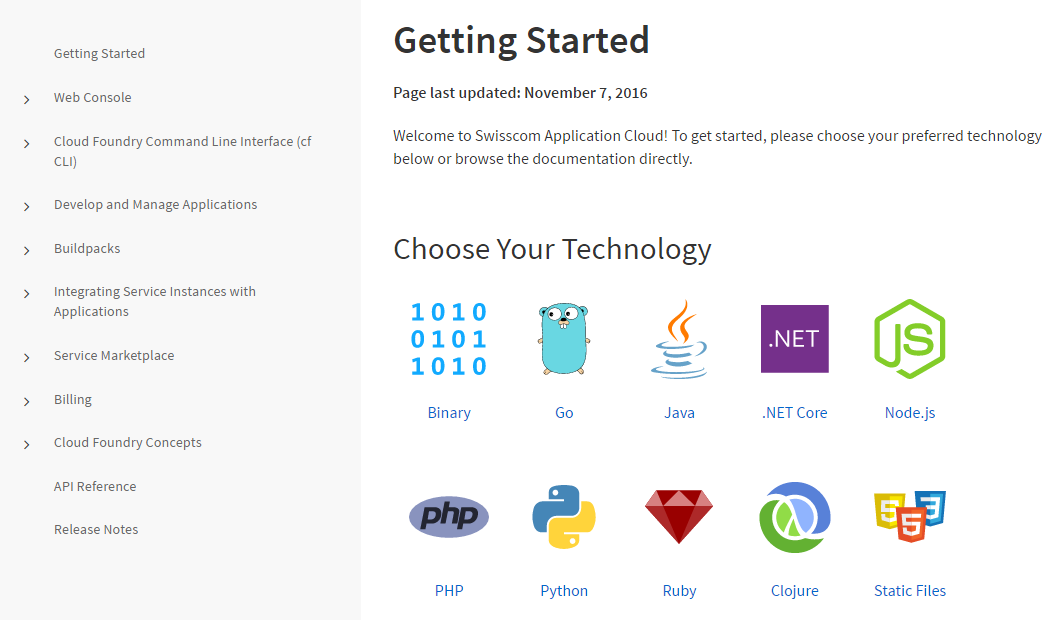
\includegraphics[width=0.65\columnwidth, valign=T]{images/image1.png}\\ \hline
Als allererstes benötigt man das Cloud Foundry Command Line Interface. Auf der Webseite sind Beschreibungen für die Installation unter Linux/Macintosh/Windows zu finden. (Windows in dieser Anleitung)&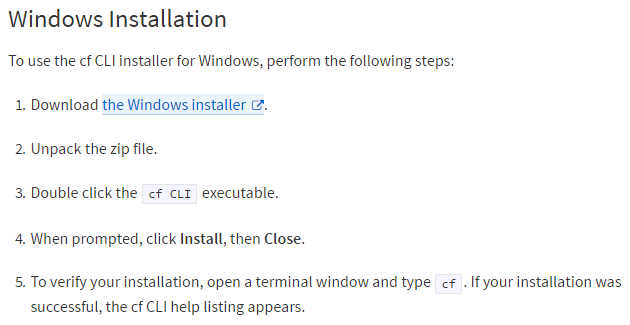
\includegraphics[width=0.65\columnwidth, valign=T]{images/image2.png} \\ \hline
\end{tabular}
\end{table}
\chapter{OSSM-Definition}
\chapter{Cloud Computing Patterns}
\chapter{Self-Information}
\chapter{Preisrecherche}
\chapter{Preisvergleich Hosting vs IaaS vs PaaS}
\chapter{Twelve-Factor Apps}

